\documentclass[10pt,a4paper]{scrartcl}
\usepackage[utf8]{inputenc}
\usepackage{amsmath}
\usepackage{amsfonts}
\usepackage{amssymb}
\usepackage[left=2cm,right=2cm,top=1cm,bottom=1cm]{geometry}
\usepackage{graphicx}

\title{Wegbeschreibung Section77}
\subtitle{Eröffnung Mitmachwerkstatt}

\begin{document}
\date{\vspace{-3em}}
\maketitle


\section*{Du kommst mit dem Auto?}
Fahre zum Bahnhof Offenburg (Hauptstraße 1, 77652 Offenburg). Parkmöglichkeiten gibt es auf dem Parkstreifen gegenüber und auf den offiziellen DB-Parkplätzen des Bahnhofs (P1 Rheinstraße und P2 Rammersweierstraße). \\

\section*{Du kommst mit der Bahn?} 
Fahre zum Bahnhof Offenburg und verlasse den Bahnhof auf der Westseite (Richtung Innenstadt). Am Ausgang nach rechts abbiegen und der Hauptstraße ca. 250m nach Norden folgen. \\

\section*{Du kommst mit dem Bus?}
Fahre bis zur Haltestelle "Offenburg Bahnhof / ZOB", von dort der Hauptstraße 300m nach Norden folgen. Die Haltestelle wird von allen Stadtbuslinien in Offenburg und allen Regionalbuslinien, die nach Offenburg fahren, bedient.

\vspace{5em}
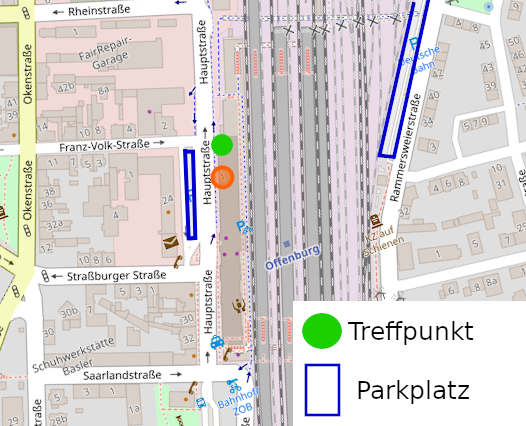
\includegraphics{./location.png}
\end{document}
